
\section{McSat: An extension of SMT Solvers}

\subsection{Introduction}


Mcsat is an extension of usual SMT solvers, introduced in~\cite{VMCAI13} and~\cite{FMCAD13}.
In usual SMT Solvers, interaction between the core SAT Solver and the Theory is pretty limited~:
the SAT Solver make boolean decision, and sends them to the theory, whose role is in return to
stop the SAT Solver as soon as the current set of assumptions is incoherent. This means
that the information that theories can give the SAT Solver is pretty limited, and furthermore
it limits the ability of theories to guide the proof search.

While it appears to leave a reasonably simple job to the theory, since it completely
hides the propositional structure of the problem, this simple interaction between the
SAT Solver and the theory makes it harder to combine multiple theories into one. Usual
techniques for combining theories in SMT solvers typically require to keep track of
equality congruence classes and require of theories to propagate any equality they discover.

McSat extends the SAT paradigm by allowing more exchange of information between the theory
and the SAT Solver. This is achieved by allowing the solver to not only decide on the truth value
of atomic propositions, but also to decide assignments for terms that appear in the problem.
For instance, if the SAT Solver assumes a formula $x = 0$,
an arithmetic theory could propagate to the SAT Solver that the formula $x < 1$ must also hold,
instead of waiting for the SAT Solver to guess the truth value of $x < 1$ and then
inform the SAT Solver that the conjunction~: $x = 0 \land \neg x < 1$ is incoherent.

This exchange of information between the SAT Solver and the theories results in
the construction of a model throughout the proof search (which explains the name
Model Constructing SAT).

\subsection{SMT Solver architecture}

We can represent a simplified version of the information flow (not taking into
account backtracking) of usual SMT Solvers, using the graph in fig~\ref{fig:smt_flow}.
In a pure Sat solver, the solver starts by doing
boolean propagation until no more literal can be propagated, at which point it
makes a decision and assign a truth value to a literal not yet assigned. It then
loops to its starting point and does boolean propagation. In an SMT solver,
after each propagation and decision, the solver sends the newly assigned literals
to the theory. The theory then has the possibility to declare the current set of
literals incoherent, and give the solver a tautology in which all literals are currently
assigned to $\bot$, thus prompting the solver to backtrack.

\begin{figure}
  \begin{center}
    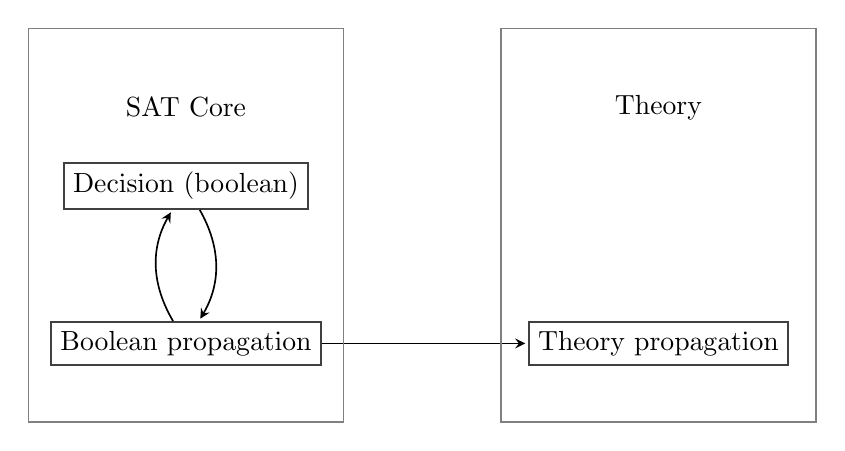
\begin{tikzpicture}[
        ->, % Arrow style
        > = stealth, % arrow head style
        shorten > = 1pt, % don't touch arrow head to node
        node distance = 2cm, % distance between nodes
        semithick, % line style
        auto
      ]

      \tikzstyle{state}=[rectangle,draw=black!75]

      \node (sat) {SAT Core};
      \node (th) [right of=sat, node distance=6cm] {Theory};
      \node[state] (d) [below of=sat, node distance=1cm] {Decision (boolean)};
      \node[state] (bp) [below of=d, node distance=2cm] {Boolean propagation};
      \node[state] (tp) [right of=bp, node distance=6cm] {Theory propagation};

      \draw (d) edge [bend left=30] (bp);
      \draw (bp) edge [bend left=30] (d);
      \draw (bp) edge (tp);

      \draw[black!50] (-2,1) rectangle (2,-4);
      \draw[black!50] (4,1) rectangle (8,-4);

    \end{tikzpicture}
  \end{center}
  \caption{Simplified SMT Solver architecture}\label{fig:smt_flow}
\end{figure}

The main addition of McSat is that when the solver makes a decision, instead of
being restricted to making boolean assignment of formulas, the solver now can
decide to assign a value to a term belonging to one of the literals. In order to do so,
the solver first chooses a term that has not yet been assigned, and then asks
the theory for a possible assignment. Like in usual SMT Solvers, a McSat solver
only exchange information with one theory, but, as we will see, combination
of theories into one becomes easier in this framework.

Since terms have assignments, the theory can now easily do useful and efficient
propagation of formulas implied by the current assignments.
The information flow then looks like fig~\ref{fig:mcsat_flow}.
For a more detailed presentation, see~\cite{FMCAD13} and~\cite{VMCAI13}.

\begin{figure}
  \begin{center}
    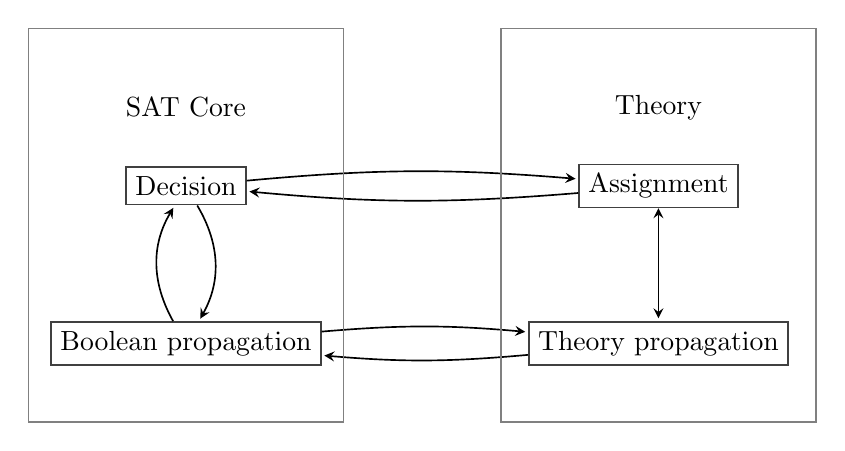
\begin{tikzpicture}[
        ->, % Arrow style
        > = stealth, % arrow head style
        shorten > = 1pt, % don't touch arrow head to node
        node distance = 2cm, % distance between nodes
        semithick, % line style
        auto
      ]

      \tikzstyle{state}=[rectangle,draw=black!75]

      \node (sat) {SAT Core};
      \node (th) [right of=sat, node distance=6cm] {Theory};
      \node[state] (d) [below of=sat, node distance=1cm] {Decision};
      \node[state] (ass) [right of=d, node distance=6cm] {Assignment};
      \node[state] (bp) [below of=d, node distance=2cm] {Boolean propagation};
      \node[state] (tp) [right of=bp, node distance=6cm] {Theory propagation};

      \draw (bp)[right] edge [bend left=5] (tp);
      \draw (tp) edge [bend left=5] (bp);
      \draw (bp) edge [bend left=30] (d);
      \draw (ass) edge [bend left=5] (d);
      \draw (d) edge [bend left=5] (ass);
      \draw (d) edge [bend left=30] (bp);
      \draw[<->] (ass) edge (tp);

      \draw[black!50] (-2,1) rectangle (2,-4);
      \draw[black!50] (4,1) rectangle (8,-4);

    \end{tikzpicture}
  \end{center}
  \caption{Simplified McSat Solver architecture}\label{fig:mcsat_flow}
\end{figure}

\subsection{Expected theory invariants}

In the following, we write $\mathbb{E}$ for the (infinite) set of first-order
expressions.

During proof search are maintained a set of assertions $\mathcal{S}$
and a partial assignment $\sigma$ as a involution of $\mathbb{E}$,
with only a finite number of $x \in \mathbb{E}$ such that $\sigma(x) \neq x$.
We say that $\mathcal{S}$ is coherent with $\sigma$ iff for every $\varphi \in \mathcal{S}$,
$\varphi\sigma$ is satisfiable (independently from the rest of the formulas in $\mathcal{S}$).
Intuitively, this represents the fact that the substitution $\sigma$ does not imply any
ground contradictions.

A theory then has to ensure that for every expression $e \in \mathbb{E}$
there exists $v \in \mathbb{E}$ such that $\mathcal{S}$ is coherent with
$\sigma \cup \{ e \rightarrow v \}$\footnote{Note that in particular, this implies
that $\mathcal{S}$ is coherent with $\sigma$}. As soon as that is not the case, the theory
should inform the SAT Solver to backtrack, since the current branch is clearly not satisfiable.
If we reach the point where all expressions of the problem have been assigned, then we
have a ground model for the current set of assertions, which is then also a model
of the input problem.

Of interest if the fact that theories that respect this invariant can easily be combined
to create a theory that also respect this invariant, as long as for any expression $e$,
there is exactly one theory responsible for finding an assignement for $e$\footnote{this
correspond to the usual criterion for combining SMT theories which is that they do not
share symbols other than equality.}.

